\documentclass{beamer}

\mode<presentation> {\usetheme{Frankfurt}}

\usepackage{graphicx} % Allows including images
\usepackage{booktabs} % Allows the use of \toprule, \midrule and \bottomrule in tables
\graphicspath{ {./images/} }

\setbeamertemplate{navigation symbols}{}

%----------------------------------------------------------------------------------------
%	TITLE PAGE
%----------------------------------------------------------------------------------------

\title[Short title]{IDE customization} % The short title appears at the bottom of every slide, the full title is only on the title page

\author{David Nápravník} % Your name
\institute[mff] % Your institution as it will appear on the bottom of every slide, may be shorthand to save space
{
Charles University \\ % Your institution for the title page
\medskip
\textit{ebrithil@nogare.cz} % Your email address
}
\date{\today} % Date, can be changed to a custom date

\begin{document}

\begin{frame}
\titlepage % Print the title page as the first slide
\end{frame}

%----------------------------------------------------------------------------------------
%	PRESENTATION SLIDES
%----------------------------------------------------------------------------------------

\section{introduction}

\begin{frame}
\frametitle{Motivation}
\begin{itemize}
\item work less do more (JQuery)
\item less mistakes
\item better orientation
\end{itemize}
\end{frame}


\section{packages}
\begin{frame}
\frametitle{Making package}
\textbf{nmp package}\\
writen in JS or TS
\begin{block}{import library}
import * as vscode from 'vscode';
\end{block}

\begin{block}{VS Code API}
commands.registerCommand('extension.sayHello', () =$>$ \{\\
~~~~window.showInformationMessage('Hello World!');\\
\});
\end{block}
\end{frame}

\begin{frame}
\frametitle{Installation}
\begin{block}{where are extensions stored}
\$HOME/.vscode/extensions/myextension
\end{block}
\begin{block}{install in shell}
code myExtensionFolder/myExtension.vsix
\end{block}
install inside IDE under package browser
\end{frame}

\begin{frame}
\frametitle{Look customize}
\textbf{theme}
\begin{itemize}
\item background
\item color of components
\end{itemize}
\textbf{icons}\\
\textbf{make it stupidly overpowered}\\
\textit{~~~~eg. vscode-spotify}
\end{frame}


\section{syntax}
\begin{frame}
\frametitle{Color}
\textbf{Bracket Pair Colorizer 2}\\
\textbf{Better Comments}\\
\textbf{Color Highlight}

\end{frame}

\begin{frame}
\frametitle{Indent}
\textbf{Readable Indent}\\
\textbf{indent-rainbow}

\end{frame}

\begin{frame}
\frametitle{Minimap}
not default in all IDEs\\
separated customization for minimap\\
\textit{~~~~eg. select highlight in minimap}
\end{frame}

\begin{frame}
\frametitle{Git history}
\textbf{GitLens - Git supercharged}
\end{frame}


\section{write faster}
\begin{frame}
\frametitle{IntelliSense}
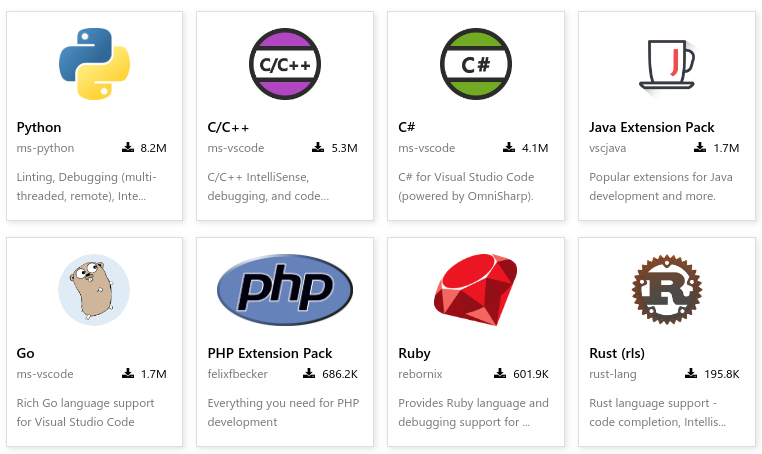
\includegraphics[scale=0.4]{images/intelisense.png}
Path Intellisense
\end{frame}

\begin{frame}
\frametitle{Code snippets}
for every language one package\\
depends on extension of file (.js)
\begin{block}{example}
    log $\rightarrow$ console.log(cursor here)
\end{block}
\end{frame}

\begin{frame}
\frametitle{Beautify}
help with:
\begin{itemize}
\item indent based on brackets
\item spaces in math
\item split lines by content
\end{itemize}
can be envoked with file save\\
can be customized\\
~~~~eg. indent with tabs / spaces (and number of spaces)
\end{frame}

\begin{frame}
\frametitle{Keyshortcuts}
shown in menu $->$ easy to learn\\
can be added in \textit{keybindings.json}
\end{frame}

\section{after coding}
\begin{frame}
\frametitle{Live server}
run server for html and JS testing\\
AJAX can be send\\
with extension can debug inside chrome
\end{frame}

\begin{frame}
\frametitle{Docker package}
control docker from IDE\\
inspect containers\\
get info about running container
\end{frame}


\section{end}
\begin{frame}
\frametitle{Sync}
sync settings, keybinds and packages\\
\textbf{Settings Sync}\\
~~~~synced over git:gist
\end{frame}

\begin{frame}
\Huge{\centerline{Questions?}}
\end{frame}

\begin{frame}
\Huge{\centerline{The End}}
\end{frame}

\end{document}